\chapter{Electrochemical Cells and Electrolysis}\label{ch:g12:cells-and-electrolysis}

A phone shows 1 \% on a winter evening and dies. Plugged in overnight, it
is full again by morning. Inside its battery the same \omterm{def:g7:chemical-reactions:reaction}{chemical reaction}
runs one way during the day, giving out electrical energy, and is driven
the other way at night by the charger. A \omterm{def:g11:redox:reaction}{redox reaction} becomes a source
of electricity when its \omterm{def:g9:inside-the-atom:nucleus}{electrons} are made to travel through a wire;
and electricity, pushed through a solution, can force a \omterm{def:g11:redox:reaction}{redox reaction}
that would never happen by itself.

\begin{recall}
\omterm{def:g11:redox:oxidant}{Oxidants} gain \omterm{def:g9:inside-the-atom:nucleus}{electrons}, \omterm{def:g11:redox:oxidant}{reductants} lose them; \omterm{def:g11:redox:couple}{half-equations}, \omterm{def:g11:redox:couple}{redox
couples} and \omterm{def:g11:redox:reaction}{redox reactions} (\cref{ch:g11:redox}). A system evolves until
$Q = K$ (\cref{ch:g12:equilibrium}). Solutions of \omterm{def:g9:ions:ion}{ions} conduct
(\cref{ch:g9:ions}); the \omterm{def:g10:the-mole:amount}{mole} and the \omterm{def:g10:the-mole:avogadro}{Avogadro constant}
(\cref{ch:g10:the-mole}).
\end{recall}

\begin{omfigure}
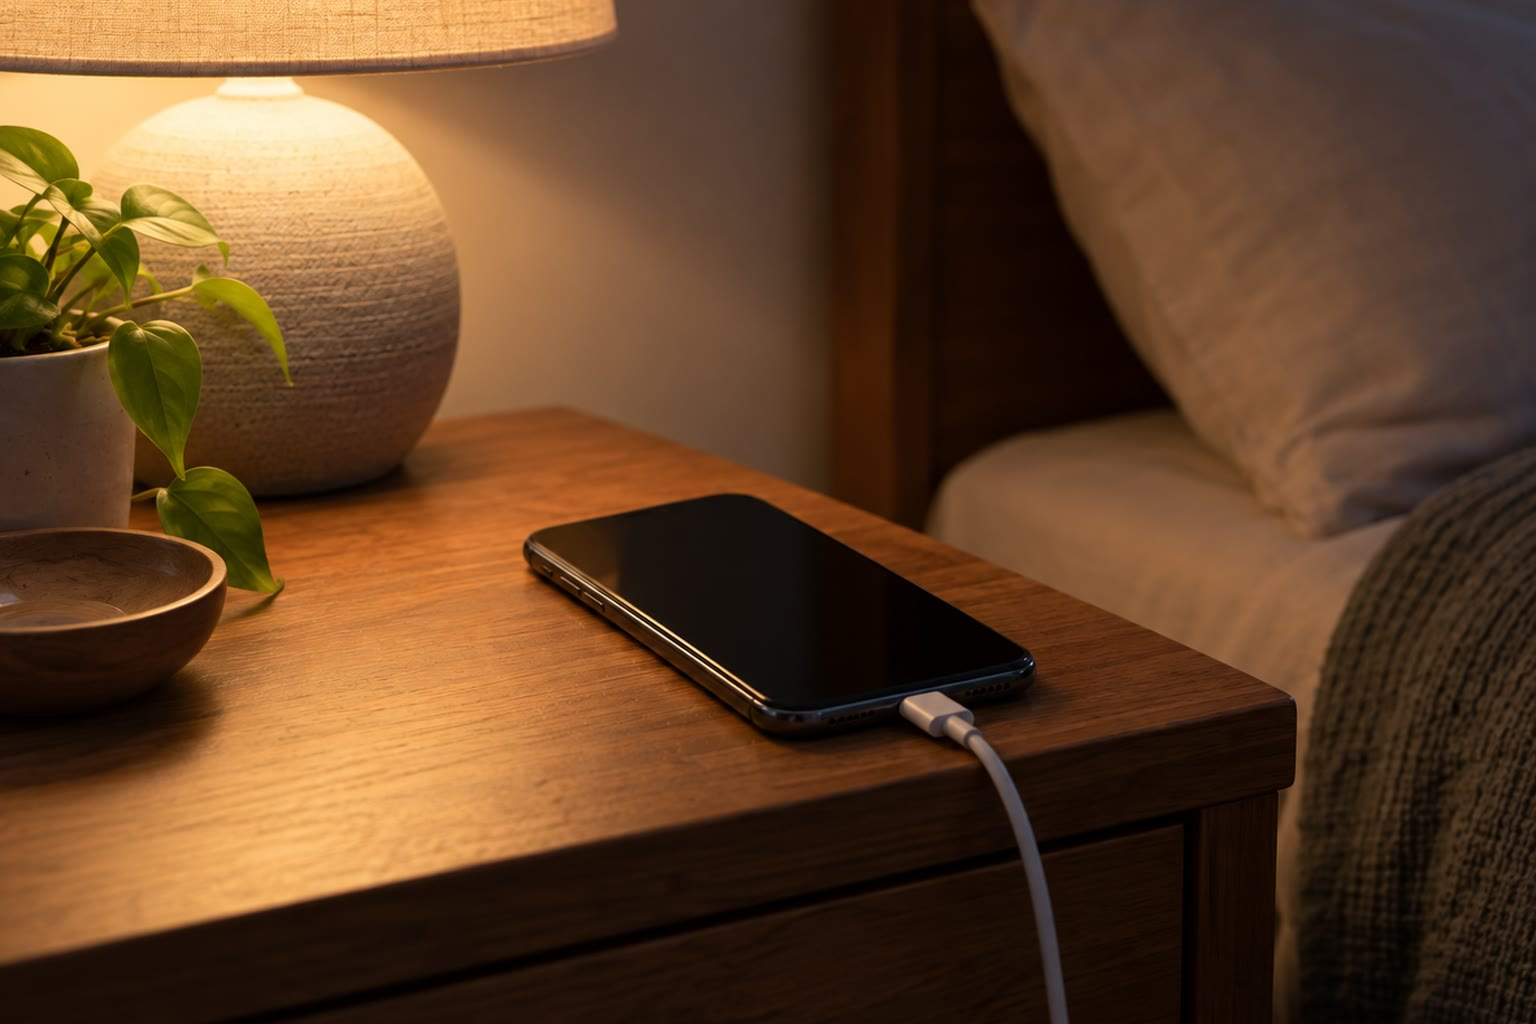
\includegraphics[width=0.45\linewidth]{images/book1/ai/g12-phone-charging.jpg}

{\small Charging a phone: a reaction driven backwards overnight.}
\end{omfigure}

\section{A redox reaction split in two}

When a zinc strip is dipped in copper sulfate solution, zinc is oxidised
and copper \omterm{def:g9:ions:ion}{ions} are reduced at the surface of the strip,
\ce{Zn + Cu^{2+} -> Zn^{2+} + Cu}: the \omterm{def:g9:inside-the-atom:nucleus}{electrons} pass directly from \omterm{def:g9:periodic-table-first-look:metal}{metal}
to \omterm{def:g9:ions:ion}{ions}, and the energy is lost as a little heat. Separate the two
halves, and join them by a wire: the \omterm{def:g9:inside-the-atom:nucleus}{electrons} must now travel through
the wire, and can light a lamp on the way.

\begin{definition}[Electrochemical cell, half-cell, salt bridge]\label{def:g12:cells-and-electrolysis:cell}
An \emph{electrochemical cell}\index{electrochemical cell} produces
electrical energy from a \omterm{def:g11:redox:reaction}{redox reaction} whose \omterm{def:g11:redox:oxidation}{oxidation} and \omterm{def:g11:redox:oxidation}{reduction} take
place in two separate compartments. Each compartment, a \omterm{def:g9:periodic-table-first-look:metal}{metal} electrode
dipped in a solution of its \omterm{def:g9:ions:ion}{ions}, is a
\emph{half-cell}\index{half-cell}. A \emph{salt bridge}\index{salt bridge},
a tube or a paper strip soaked in a solution of \omterm{def:g9:ions:ion}{ions}, joins the two
solutions and closes the circuit while keeping them apart.
\end{definition}

\begin{definition}[Anode, cathode]\label{def:g12:cells-and-electrolysis:anode}
The electrode where an \omterm{def:g11:redox:oxidation}{oxidation} takes place is the
\emph{anode}\index{anode}; the electrode where a \omterm{def:g11:redox:oxidation}{reduction} takes place
is the \emph{cathode}\index{cathode}.
\end{definition}

\begin{omfigure}
\begin{tikzpicture}[font=\small, scale=1.25]
  \pic[transform shape] at (0,0) {beaker={0.7}{black!6}};
  \pic[transform shape] at (4,0) {beaker={0.7}{cyan!70!blue!35}};
  \pic[transform shape] (zn) at (-0.3,0.25) {electrode={black!30}};
  \pic[transform shape] (cu) at (4.3,0.25) {electrode={orange!70!brown}};
  \pic[transform shape] at (0.35,0.6) {saltbridge={3.3}};
  \pic[transform shape] (v) at (2,3.9) {meter={1.10 V}};
  \draw[black!70, thick] (zn-top) |- (1.0,3.4) -| (v-a);
  \draw[black!70, thick] (cu-top) |- (3.0,3.4) -| (v-b);
  \draw[->, omProp, very thick] (0.2,3.55) -- (1.0,3.55);
  \draw[->, omProp, very thick] (3.0,3.55) -- (3.8,3.55);
  \node[omProp, font=\footnotesize] at (0.6,3.75) {$e^-$};
  \node[omProp, font=\footnotesize] at (3.4,3.75) {$e^-$};
  \node[anchor=north, align=center] at (-0.2,-0.15) {anode ($-$): zinc\\ \ce{Zn -> Zn^{2+} + 2e-}};
  \node[anchor=north, align=center] at (4.2,-0.15) {cathode ($+$): copper\\ \ce{Cu^{2+} + 2e- -> Cu}};
  \node[font=\footnotesize, anchor=east, align=right] at (-0.95,0.7) {\ce{Zn^{2+}}\\ \ce{SO4^{2-}}};
  \node[font=\footnotesize, anchor=west, align=left] at (4.95,0.7) {\ce{Cu^{2+}}\\ \ce{SO4^{2-}}};
  \node[font=\footnotesize, align=center] at (2,2.45) {salt bridge\\ (\ce{K+}, \ce{NO3-})};
\end{tikzpicture}

{\small The Daniell cell. \omterm{def:g9:inside-the-atom:nucleus}{Electrons} leave the zinc \omterm{def:g12:cells-and-electrolysis:anode}{anode} through the
wire and enter the copper \omterm{def:g12:cells-and-electrolysis:anode}{cathode}; in the \omterm{def:g12:cells-and-electrolysis:cell}{salt bridge}, \omterm{def:g9:ions:ion}{ions} move to keep
each solution neutral.}
\end{omfigure}

\begin{proposition}[Where the electrons go]\label{prop:g12:cells-and-electrolysis:flow}
In a cell delivering current, \omterm{def:g9:inside-the-atom:nucleus}{electrons} leave the cell by the \omterm{def:g12:cells-and-electrolysis:anode}{anode},
where they are released by the \omterm{def:g11:redox:oxidation}{oxidation}, travel through the external
circuit, and enter by the \omterm{def:g12:cells-and-electrolysis:anode}{cathode}, where they are taken by the
\omterm{def:g11:redox:oxidation}{reduction}. The \omterm{def:g12:cells-and-electrolysis:anode}{anode} is the negative terminal, the \omterm{def:g12:cells-and-electrolysis:anode}{cathode} the positive
one. Inside, the current is carried by \omterm{def:g9:ions:ion}{ions}: \omterm{def:g9:ions:ion}{cations} move towards the
\omterm{def:g12:cells-and-electrolysis:anode}{cathode}, \omterm{def:g9:ions:ion}{anions} towards the \omterm{def:g12:cells-and-electrolysis:anode}{anode}.
\end{proposition}

\begin{proof}
The \omterm{def:g11:redox:oxidation}{oxidation} produces \omterm{def:g9:inside-the-atom:nucleus}{electrons} at the \omterm{def:g12:cells-and-electrolysis:anode}{anode}; the \omterm{def:g11:redox:oxidation}{reduction} consumes
them at the \omterm{def:g12:cells-and-electrolysis:anode}{cathode}; the wire is the only path between the two. Each
solution would otherwise become charged, which the \omterm{def:g9:ions:ion}{ions} of the bridge
prevent.
\end{proof}

\begin{method}[Describing a cell]\label{met:g12:cells-and-electrolysis:describe}
\begin{enumerate}
  \item Write the overall \omterm{def:g11:redox:reaction}{redox reaction} that takes place spontaneously.
  \item Split it into two \omterm{def:g11:redox:couple}{half-equations}: the \omterm{def:g11:redox:oxidation}{oxidation} (\omterm{def:g12:cells-and-electrolysis:anode}{anode}) and the
        \omterm{def:g11:redox:oxidation}{reduction} (\omterm{def:g12:cells-and-electrolysis:anode}{cathode}).
  \item Mark the polarity: \omterm{def:g12:cells-and-electrolysis:anode}{anode} $-$, \omterm{def:g12:cells-and-electrolysis:anode}{cathode} $+$; the direction of the
        \omterm{def:g9:inside-the-atom:nucleus}{electrons} in the wire (\omterm{def:g12:cells-and-electrolysis:anode}{anode} to \omterm{def:g12:cells-and-electrolysis:anode}{cathode}) and of the current
        (\omterm{def:g12:cells-and-electrolysis:anode}{cathode} to \omterm{def:g12:cells-and-electrolysis:anode}{anode}).
  \item Describe the motion of the \omterm{def:g9:ions:ion}{ions} in the bridge.
\end{enumerate}
\end{method}


\begin{history}[Volta's pile, 1800]
In 1800 the physicist Alessandro Volta stacked discs of two different
\omterm{def:g9:periodic-table-first-look:metal}{metals}, zinc and copper or silver, separated by pieces of cloth soaked in
brine, and obtained a steady electric current: the first battery. It
gave physicists their first continuous source of electricity, and
chemists a new tool: within a few years \omterm{def:g12:cells-and-electrolysis:electrolysis}{electrolysis} had isolated sodium
and potassium for the first time.
\end{history}

\begin{omfigure}
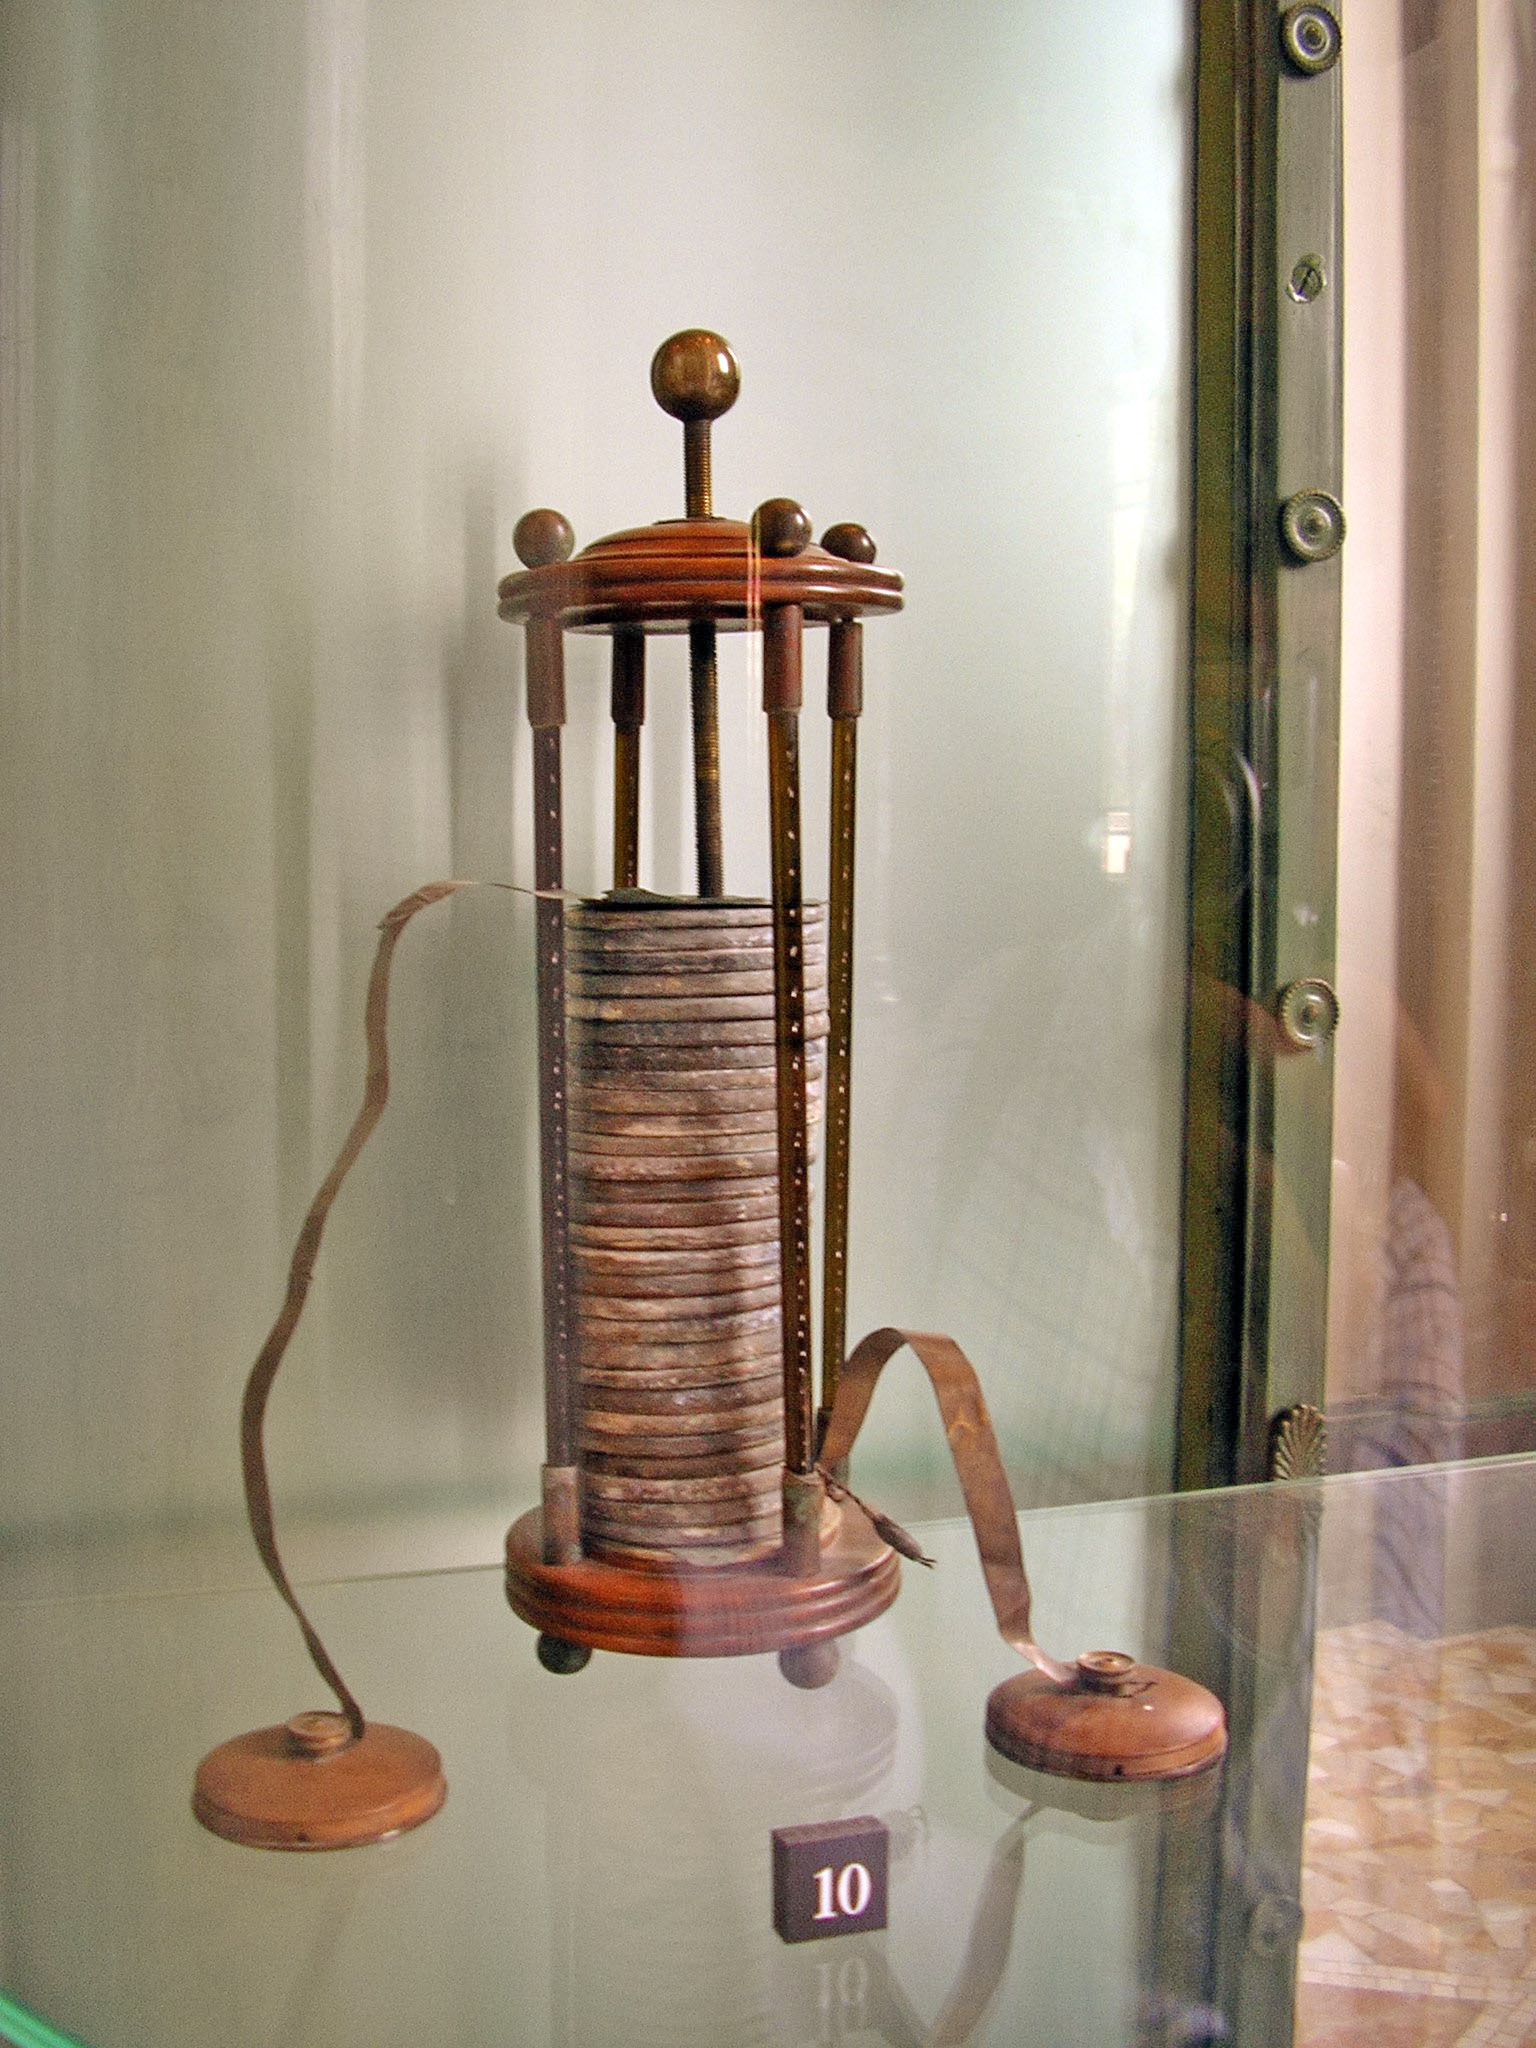
\includegraphics[width=0.24\linewidth]{images/book1/volta-pile.jpg}

{\small A voltaic pile in a museum. Photo GuidoB, CC BY-SA 3.0.}
\end{omfigure}

\section{The voltage of a cell}

\begin{definition}[Cell voltage]\label{def:g12:cells-and-electrolysis:emf}
The \emph{cell voltage}\index{cell voltage} is the voltage measured
between the terminals of a cell delivering no current (open circuit),
with a voltmeter; it is positive when the voltmeter's positive terminal
is on the \omterm{def:g12:cells-and-electrolysis:anode}{cathode}.
\end{definition}

\begin{example}[The Daniell cell]\label{ex:g12:cells-and-electrolysis:daniell}
% ledger: e0:Cu, e0:Zn, emf:Daniell
With both solutions at \qty{1}{mol/L}, the Daniell cell gives
\qty{1.10}{V}. How such a voltage is predicted from tables of electrode
potentials is shown in the Year 1 volume.
\end{example}

\begin{remark}[Why a cell runs down]\label{rem:g12:cells-and-electrolysis:runs-down}
The reaction of the cell, \ce{Zn + Cu^{2+} -> Zn^{2+} + Cu}, has a very
large constant $K$. While the cell works, $Q = [\ce{Zn^{2+}}]/[\ce{Cu^{2+}}]$
grows, and the reaction keeps running as long as $Q < K$. When a
\omterm{def:g7:chemical-reactions:reactant}{reactant} runs out (the zinc, or the copper \omterm{def:g9:ions:ion}{ions}), the current stops: the
cell is ``flat''.
\end{remark}

\section{Charge and capacity}

\begin{definition}[Faraday constant, capacity]\label{def:g12:cells-and-electrolysis:capacity}
The \emph{Faraday constant}\index{Faraday constant} $F$ is the electric
charge of one \omterm{def:g10:the-mole:amount}{mole} of \omterm{def:g9:inside-the-atom:nucleus}{electrons}, $F = N_A e = \qty{96485}{C/mol}$. The
\emph{capacity}\index{capacity} of a cell is the largest electric charge
it can deliver, often given in ampere-hours: $\qty{1}{A.h} = \qty{3600}{C}$.
\end{definition}

\begin{proposition}[Charge and amount of electrons]\label{prop:g12:cells-and-electrolysis:charge}
% ledger: const:F, const:NA, const:e
A current $I$ flowing for a time $\Delta t$ carries the charge
$Q = I\,\Delta t$, that is an amount of \omterm{def:g9:inside-the-atom:nucleus}{electrons}
\[
  n(e^-) = \frac{Q}{F} = \frac{I\,\Delta t}{F} .
\]
\end{proposition}

\begin{proof}
Each \omterm{def:g9:inside-the-atom:nucleus}{electron} carries the elementary charge $e$; $n$ \omterm{def:g10:the-mole:amount}{moles} of \omterm{def:g9:inside-the-atom:nucleus}{electrons}
carry $n N_A e = n F$.
\end{proof}

\begin{example}[Capacity of a Daniell cell]\label{ex:g12:cells-and-electrolysis:capacity}
% ledger: aw:Zn, const:F
The zinc electrode holds \qty{6.5}{g} of zinc that can react, that is
$6.5/65.4 = \qty{0.099}{mol}$. Each zinc \omterm{def:g7:atoms-and-molecules:atom}{atom} gives two \omterm{def:g9:inside-the-atom:nucleus}{electrons}:
$n(e^-) = \qty{0.199}{mol}$, so $Q = 0.199 \times 96485 = \qty{1.9e4}{C}$,
about $\qty{1.9e4}{}/3600 = \qty{5.3}{A.h}$, if the copper \omterm{def:g9:ions:ion}{ions} do not
run out first.
\end{example}

\section{Electrolysis}

\begin{definition}[Electrolysis, accumulator]\label{def:g12:cells-and-electrolysis:electrolysis}
An \emph{electrolysis}\index{electrolysis} is a \omterm{def:g11:redox:reaction}{redox reaction} forced by
an electrical generator, in the direction opposite to the one it would
take by itself. An \emph{accumulator}\index{accumulator} is a cell that
can be recharged: during charging, the generator drives its reaction
backwards, as an electrolysis.
\end{definition}

\begin{inthelab}[Electrolysis of water]
Two electrodes dip in water made conducting with a little sodium
sulfate, each under an inverted test tube full of the solution. With a
generator of a few volts, bubbles rise from both electrodes: at the
\omterm{def:g12:cells-and-electrolysis:anode}{cathode} (connected to the $-$ terminal) dihydrogen, at the \omterm{def:g12:cells-and-electrolysis:anode}{anode}
dioxygen, twice as much of the first as of the second. A lighted splint
pops in the first gas; a glowing splint relights in the second.
\end{inthelab}

\begin{omfigure}
\begin{tikzpicture}[font=\small, scale=1.2]
  % a trough of water, two inverted tubes standing in it
  \fill[omWater] (-1.4,0) rectangle (1.4,1.1);
  \foreach \x/\g in {-0.6/1.2, 0.6/0.6} {
    \fill[omWater] (\x-0.18,0.3) rectangle (\x+0.18,2.9);
    \fill[white] (\x-0.18,{2.9-\g}) rectangle (\x+0.18,2.9);
    \fill[white] (\x,2.9) circle (0.18);
    \draw[om glass] (\x-0.18,0.3) -- (\x-0.18,2.9) arc[start angle=180, end angle=0, radius=0.18] -- (\x+0.18,0.3);
  }
  \draw[om glass] (-1.5,1.25) -- (-1.4,1.15) -- (-1.4,0) -- (1.4,0) -- (1.4,1.15) -- (1.5,1.25);
  \fill[black!55] (-0.65,0) rectangle (-0.55,0.6);
  \fill[black!55] (0.55,0) rectangle (0.65,0.6);
  \node[draw, fill=white, minimum width=1.6cm, minimum height=0.45cm, font=\footnotesize] (g) at (0,-0.75) {generator};
  \draw[black!70, thick] (-0.6,0) -- (-0.6,0 |- g.north);
  \draw[black!70, thick] (0.6,0) -- (0.6,0 |- g.north);
  \node[font=\footnotesize] at (-0.78,-0.3) {$-$};
  \node[font=\footnotesize] at (0.78,-0.3) {$+$};
  \node[anchor=east, align=right] at (-0.95,2.5) {dihydrogen\\ (cathode)};
  \node[anchor=west, align=left] at (0.95,2.5) {dioxygen\\ (anode)};
\end{tikzpicture}

{\small \omterm{def:g12:cells-and-electrolysis:electrolysis}{Electrolysis} of water: twice as much dihydrogen as dioxygen
collects above the electrodes.}
\end{omfigure}


\begin{example}[Water, split]\label{ex:g12:cells-and-electrolysis:water}
At the \omterm{def:g12:cells-and-electrolysis:anode}{cathode}: \ce{2H2O + 2e- -> H2 + 2OH-}; at the \omterm{def:g12:cells-and-electrolysis:anode}{anode}:
\ce{6H2O -> O2 + 4H3O+ + 4e-}. For four \omterm{def:g9:inside-the-atom:nucleus}{electrons}, two \omterm{def:g7:atoms-and-molecules:molecule}{molecules} of
dihydrogen and one of dioxygen, while the \omterm{def:g9:ions:ion}{ions} \ce{H3O+} and \ce{OH-}
formed at the two electrodes recombine into water: overall
\ce{2H2O -> 2H2 + O2}, the
reverse of the \omterm{def:g4:what-a-fire-needs:burning}{combustion} of hydrogen, which needs energy to happen.
\end{example}

\begin{method}[Mass deposited by an electrolysis]\label{met:g12:cells-and-electrolysis:mass}
\begin{enumerate}
  \item Write the \omterm{def:g11:redox:couple}{half-equation} at the electrode where the \omterm{def:g9:periodic-table-first-look:metal}{metal} forms,
        for example \ce{Cu^{2+} + 2e- -> Cu}.
  \item Compute the charge $Q = I \Delta t$ and $n(e^-) = Q/F$.
  \item Divide by the number of \omterm{def:g9:inside-the-atom:nucleus}{electrons} per \omterm{def:g7:atoms-and-molecules:atom}{atom}: $n(\ce{Cu}) =
        n(e^-)/2$; then $m = n \times M$.
\end{enumerate}
\end{method}


\begin{example}[Refining copper]\label{ex:g12:cells-and-electrolysis:refining}
% ledger: aw:Cu, const:F
Impure copper from the smelter is made the \omterm{def:g12:cells-and-electrolysis:anode}{anode} of an \omterm{def:g12:cells-and-electrolysis:electrolysis}{electrolysis} cell
in copper sulfate solution, and a thin sheet of pure copper the \omterm{def:g12:cells-and-electrolysis:anode}{cathode}.
At the \omterm{def:g12:cells-and-electrolysis:anode}{anode} copper \omterm{def:g2:mixing-and-dissolving:dissolve}{dissolves}, \ce{Cu -> Cu^{2+} + 2e-}; at the \omterm{def:g12:cells-and-electrolysis:anode}{cathode}
pure copper is deposited, \ce{Cu^{2+} + 2e- -> Cu}; the impurities fall to
the bottom or stay in solution. A current of \qty{100}{A} for
\qty{24}{h} carries $Q = 100 \times 86400 = \qty{8.64e6}{C}$, that is
$n(e^-) = \qty{89.5}{mol}$, which deposits $89.5/2 = \qty{44.8}{mol}$ of
copper: \qty{2.84}{kg}.
\end{example}

\begin{omfigure}
\begin{tikzpicture}[font=\small, scale=1.25]
  \pic[transform shape] at (0,0) {beaker={0.75}{cyan!70!blue!35}};
  \pic[transform shape] (an) at (-0.4,0.2) {electrode={orange!40!brown!80!black}};
  \pic[transform shape] (ca) at (0.4,0.2) {electrode={orange!80!brown}};
  \foreach \p in {(-0.6,0.08),(-0.5,0.12),(-0.3,0.07),(-0.2,0.1)} \fill[black!55] \p circle (0.03);
  \node[draw, fill=white, font=\footnotesize, minimum width=1.6cm] (g) at (0,3.4) {generator};
  \draw[black!70, thick] (an-top) -- (an-top |- g.south);
  \draw[black!70, thick] (ca-top) -- (ca-top |- g.south);
  \node[font=\footnotesize] at (-0.58,2.95) {$+$};
  \node[font=\footnotesize] at (0.58,2.95) {$-$};
  \draw[omProp, thick, <-] (-0.55,1.2) -- (-1.6,1.6) node[left, align=right, text=black] {impure copper\\ anode: dissolves};
  \draw[omProp, thick, <-] (0.55,1.2) -- (1.6,1.6) node[right, align=left, text=black] {pure copper\\ cathode: grows};
  \draw[omProp, thick, <-] (-0.35,0.1) -- (-1.6,0.3) node[left, text=black] {impurities};
\end{tikzpicture}

{\small Copper refining by \omterm{def:g12:cells-and-electrolysis:electrolysis}{electrolysis}: copper passes from the impure
\omterm{def:g12:cells-and-electrolysis:anode}{anode} to the pure \omterm{def:g12:cells-and-electrolysis:anode}{cathode} through the solution.}
\end{omfigure}

\section{Batteries, accumulators and fuel cells}

Every battery is a cell, every rechargeable battery an \omterm{def:g12:cells-and-electrolysis:electrolysis}{accumulator}. A
car's lead--acid \omterm{def:g12:cells-and-electrolysis:electrolysis}{accumulator} works with lead, lead oxide and sulfuric
acid; a phone's lithium-ion \omterm{def:g12:cells-and-electrolysis:electrolysis}{accumulator} moves lithium \omterm{def:g9:ions:ion}{ions} between two
electrodes, one of graphite and one of a \omterm{def:g9:periodic-table-first-look:metal}{metal} oxide, through a liquid
or polymer electrolyte, while the \omterm{def:g9:inside-the-atom:nucleus}{electrons} go round the outside
circuit. A \omterm{def:g4:what-a-fire-needs:fuel}{fuel} cell is a cell whose \omterm{def:g7:chemical-reactions:reactant}{reactants} are fed in continuously:
a hydrogen \omterm{def:g4:what-a-fire-needs:fuel}{fuel} cell runs the reaction \ce{2H2 + O2 -> 2H2O}, the
reverse of the \omterm{def:g12:cells-and-electrolysis:electrolysis}{electrolysis} of water, and gives electricity and water.
Dihydrogen made by \omterm{def:g12:cells-and-electrolysis:electrolysis}{electrolysis} with electricity from wind or sun, then
used in \omterm{def:g4:what-a-fire-needs:fuel}{fuel} cells, is one way of storing that electricity.

\begin{omfigure}
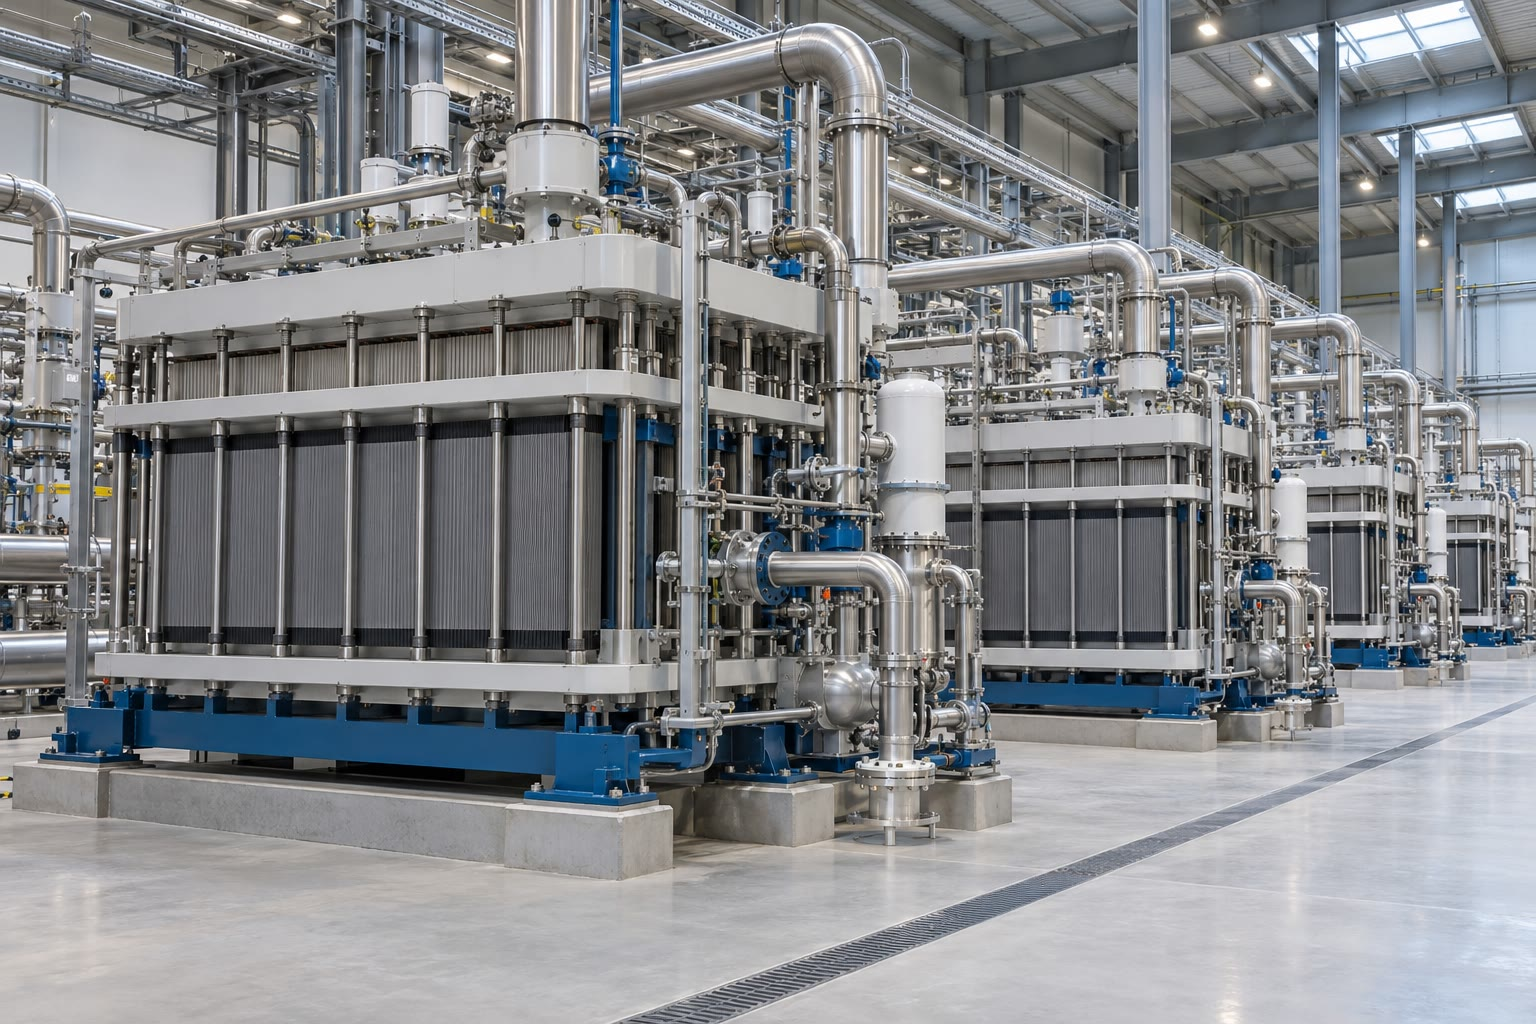
\includegraphics[width=0.48\linewidth]{images/book1/ai/g12-electrolyser-hall.jpg}

{\small An electrolyser hall: water is split into dihydrogen and
dioxygen.}
\end{omfigure}

\section{Exercises}

\begin{exercise}[$\star$]\label{exo:g12:cells-and-electrolysis:1}
In the Daniell cell, which electrode is the \omterm{def:g12:cells-and-electrolysis:anode}{anode}? The \omterm{def:g12:cells-and-electrolysis:anode}{cathode}? Write
the \omterm{def:g11:redox:couple}{half-equation} at each.
\end{exercise}

\begin{exercise}[$\star$]\label{exo:g12:cells-and-electrolysis:2}
A current of \qty{0.20}{A} flows for \qty{30}{min}. Compute the charge
carried and the amount of \omterm{def:g9:inside-the-atom:nucleus}{electrons}.
\end{exercise}

\begin{exercise}[$\star$]\label{exo:g12:cells-and-electrolysis:3}
What is the role of the \omterm{def:g12:cells-and-electrolysis:cell}{salt bridge}? What happens if it is removed?
\end{exercise}

\begin{exercise}[$\star$]\label{exo:g12:cells-and-electrolysis:4}
Convert a \omterm{def:g12:cells-and-electrolysis:capacity}{capacity} of \qty{2.5}{A.h} into coulombs.
\end{exercise}

\begin{exercise}[$\star$]\label{exo:g12:cells-and-electrolysis:5}
In an \omterm{def:g12:cells-and-electrolysis:electrolysis}{electrolysis}, is the reaction spontaneous? What supplies the
energy?
\end{exercise}

\begin{exercise}[$\star\star$]\label{exo:g12:cells-and-electrolysis:6}
A cell is made of a silver electrode in silver nitrate and a copper
electrode in copper sulfate. The voltmeter shows that \omterm{def:g9:inside-the-atom:nucleus}{electrons} leave
by the copper. Write the \omterm{def:g11:redox:couple}{half-equations}, name the \omterm{def:g12:cells-and-electrolysis:anode}{anode} and the \omterm{def:g12:cells-and-electrolysis:anode}{cathode},
and give the overall reaction.
\end{exercise}

\begin{exercise}[$\star\star$]\label{exo:g12:cells-and-electrolysis:7}
A watch battery delivers \qty{10}{\micro A} continuously for three years.
What is its \omterm{def:g12:cells-and-electrolysis:capacity}{capacity} in \si{mA.h}?
\end{exercise}

\begin{exercise}[$\star\star$]\label{exo:g12:cells-and-electrolysis:8}
A spoon is silver-plated with a current of \qty{0.50}{A} for
\qty{40}{min}, \ce{Ag+ + e- -> Ag}. What mass of silver is deposited?
\end{exercise}

\begin{exercise}[$\star\star$]\label{exo:g12:cells-and-electrolysis:9}
On the figure of the Daniell cell, give the direction of the current in
the wire, and the direction in which the \ce{K+} and \ce{NO3-} \omterm{def:g9:ions:ion}{ions} of
the bridge move.
\end{exercise}

\begin{exercise}[$\star\star$]\label{exo:g12:cells-and-electrolysis:10}
Compare a cell and an \omterm{def:g12:cells-and-electrolysis:electrolysis}{electrolysis}: the sign of the \omterm{def:g12:cells-and-electrolysis:anode}{anode}, the direction
of the reaction, the conversion of energy.
\end{exercise}

\begin{exercise}[$\star\star$]\label{exo:g12:cells-and-electrolysis:11}
In the \omterm{def:g12:cells-and-electrolysis:electrolysis}{electrolysis} of water, \qty{24}{mL} of dihydrogen are collected.
What volume of dioxygen is collected at the same time? Why?
\end{exercise}

\begin{exercise}[$\star\star\star$]\label{exo:g12:cells-and-electrolysis:12}
A Daniell cell contains \qty{5.0}{g} of zinc and \qty{100}{mL} of copper
sulfate at \qty{0.50}{mol/L}. Which \omterm{def:g7:chemical-reactions:reactant}{reactant} runs out first? What is the
\omterm{def:g12:cells-and-electrolysis:capacity}{capacity} of the cell? How long can it deliver \qty{50}{mA}?
\end{exercise}

\begin{exercise}[$\star\star\star$]\label{exo:g12:cells-and-electrolysis:13}
A battery of \qty{1.5}{V} delivers \qty{2.0}{A.h}. Compute the energy it
stores ($E = Q U$), in joules and in watt-hours.
\end{exercise}

\begin{exercise}[$\star\star\star$]\label{exo:g12:cells-and-electrolysis:14}
Water is electrolysed with \qty{2.0}{A} for \qty{1.0}{h}. Compute the
amounts, then the volumes at \qty{20}{\celsius} ($V_m = \qty{24.1}{L/mol}$),
of dihydrogen and dioxygen produced.
\end{exercise}

\begin{exercise}[$\star\star\star$]\label{exo:g12:cells-and-electrolysis:15}
In copper refining, the \omterm{def:g12:cells-and-electrolysis:anode}{anode} loses \qty{3.00}{kg} of material while the
\omterm{def:g12:cells-and-electrolysis:anode}{cathode} gains \qty{2.84}{kg} of copper. What is the percentage of copper
in the impure \omterm{def:g12:cells-and-electrolysis:anode}{anode}, assuming that only copper is oxidised at the \omterm{def:g12:cells-and-electrolysis:anode}{anode}
and the impurities simply fall off?
\end{exercise}

\section{Problem: The Phone Battery}

\begin{problem}[{Weekend problem --- what mass of lithium shuttles between
the electrodes of a \qty{4000}{mA.h} phone battery?}]
\label{pb:g12:cells-and-electrolysis:1}
% ledger: const:F, const:NA, aw:Li, dch:CH4, aw:C, aw:H
A phone battery is labelled ``\qty{3.7}{V}, \qty{4000}{mA.h}''. In a
simplified picture, during discharge each lithium \omterm{def:g7:atoms-and-molecules:atom}{atom} stored in the
graphite electrode gives one \omterm{def:g9:inside-the-atom:nucleus}{electron} and leaves as a lithium \omterm{def:g9:ions:ion}{ion},
\ce{Li -> Li+ + e-}; the \omterm{def:g9:ions:ion}{ion} crosses the electrolyte and is taken up by
the \omterm{def:g9:periodic-table-first-look:metal}{metal} oxide electrode, which gains an \omterm{def:g9:inside-the-atom:nucleus}{electron} at the same time.

\medskip
\noindent\textbf{Part I --- The cell.}
\begin{enumerate}
  \item During discharge, is the graphite electrode the \omterm{def:g12:cells-and-electrolysis:anode}{anode} or the
        \omterm{def:g12:cells-and-electrolysis:anode}{cathode}? Why?
  \item Which is the negative terminal?
  \item In which direction do the \omterm{def:g9:inside-the-atom:nucleus}{electrons} travel through the phone?
        And the lithium \omterm{def:g9:ions:ion}{ions} inside the battery?
  \item Why is this cell an \omterm{def:g12:cells-and-electrolysis:electrolysis}{accumulator}?
\end{enumerate}

\medskip
\noindent\textbf{Part II --- The charge.}
\begin{enumerate}[resume]
  \item Convert \qty{4000}{mA.h} into ampere-hours, then into coulombs.
  \item Compute the amount of \omterm{def:g9:inside-the-atom:nucleus}{electrons} this charge represents.
  \item How many \omterm{def:g9:inside-the-atom:nucleus}{electrons} is that?
  \item The phone draws on average \qty{0.25}{A}. How long does a full
        battery last?
  \item The screen shows 20 \%. What charge, in coulombs, is left?
\end{enumerate}

\medskip
\noindent\textbf{Part III --- The energy.}
\begin{enumerate}[resume]
  \item Compute the energy stored, $E = Q U$, in joules.
  \item Convert it into watt-hours.
  \item Compare with the energy released by \omterm{def:g4:what-a-fire-needs:burning}{burning} \qty{1}{g} of methane
        (\qty{55.7}{kJ}).
  \item How many full charges does \qty{1}{kW.h} of electricity give, if
        no energy were lost?
\end{enumerate}

\medskip
\noindent\textbf{Part IV --- Recharging.}
\begin{enumerate}[resume]
  \item During charging, which reaction takes place at the graphite
        electrode? Is it an \omterm{def:g11:redox:oxidation}{oxidation} or a \omterm{def:g11:redox:oxidation}{reduction}?
  \item Why is recharging an \omterm{def:g12:cells-and-electrolysis:electrolysis}{electrolysis}?
  \item The charger delivers \qty{2.0}{A}. How long does a full recharge
        take at least?
  \item What amount of lithium \omterm{def:g9:ions:ion}{ions} crosses the electrolyte during one
        full charge?
  \item Compute their mass.
  \item State the final answer: what mass of lithium shuttles between the
        electrodes in one full charge?
\end{enumerate}
\end{problem}
